\documentclass[12pt]{article}
\usepackage{graphicx}
\usepackage{amsmath}
\usepackage{amsfonts}
\usepackage{float}
\usepackage{hyperref}


\title{CNN Model Evaluation and Visualization for Architectural Heritage Classification}
\author{Mahla Entezari}
\date{Spring 2024}

\begin{document}

\maketitle

\begin{abstract}
This report discusses the implementation of a Convolutional Neural Network (CNN) model for the classification of architectural heritage images from the "Architectural Heritage Elements Image64" dataset. The project involves training a CNN model to classify images into ten categories and visualizing the feature maps generated by the model using deconvolution techniques. The performance of the model is evaluated using a confusion matrix, and insights into the model's behavior are drawn from the feature maps of the first convolutional layer.
\end{abstract}

\section{Introduction}
The recognition and classification of architectural heritage elements is a challenging task in the field of computer vision. Convolutional Neural Networks (CNNs) have proven to be highly effective in image classification tasks due to their ability to learn hierarchical representations of data. In this project, we explore the use of CNNs to classify architectural elements from the "Architectural Heritage Elements Image64" dataset, which includes ten categories such as altar, apse, bell tower, column, and others.

The objectives of this project are threefold: to build and train a CNN model, to visualize the learned feature maps using deconvolution techniques, and to explore the model's ability to generate images for specific classes.

\section{Dataset Description}
The dataset used in this project consists of 10,235 images classified into ten categories related to architectural heritage elements. These categories are:

\begin{itemize}
    \item Altar
    \item Apse
    \item Bell Tower
    \item Column
    \item Dome (Inner)
    \item Dome (Outer)
    \item Flying Buttress
    \item Gargoyle
    \item Stained Glass
    \item Vault
\end{itemize}

Each category contains images representing various architectural elements that are typically found in historical buildings. The dataset is well-suited for training CNN models due to its diverse range of images.

\section{Methodology}
\subsection{Data Preprocessing}
Data preprocessing is a crucial step in preparing the images for input into the CNN model. The preprocessing steps include:
\begin{itemize}
    \item Resizing the images to a uniform size (64x64 pixels).
    \item Normalizing the pixel values to the range [0, 1].
    \item Splitting the dataset into training and testing subsets.
\end{itemize}

Data augmentation techniques, such as random rotations and flips, were applied during training to enhance the model's ability to generalize.

\subsection{Model Architecture}
The CNN model used for this project consists of the following layers:
\begin{itemize}
    \item Convolutional layers with ReLU activation.
    \item Max-pooling layers.
    \item Fully connected (dense) layers for classification.
\end{itemize}

The model is trained using the Adam optimizer with a categorical cross-entropy loss function, suitable for multi-class classification tasks.

\subsection{Model Training}
The model was trained on a training subset of the dataset using a batch size of 32 and for 50 epochs. Various techniques such as dropout and early stopping were employed to prevent overfitting. 

\begin{figure}[H]
    \centering
    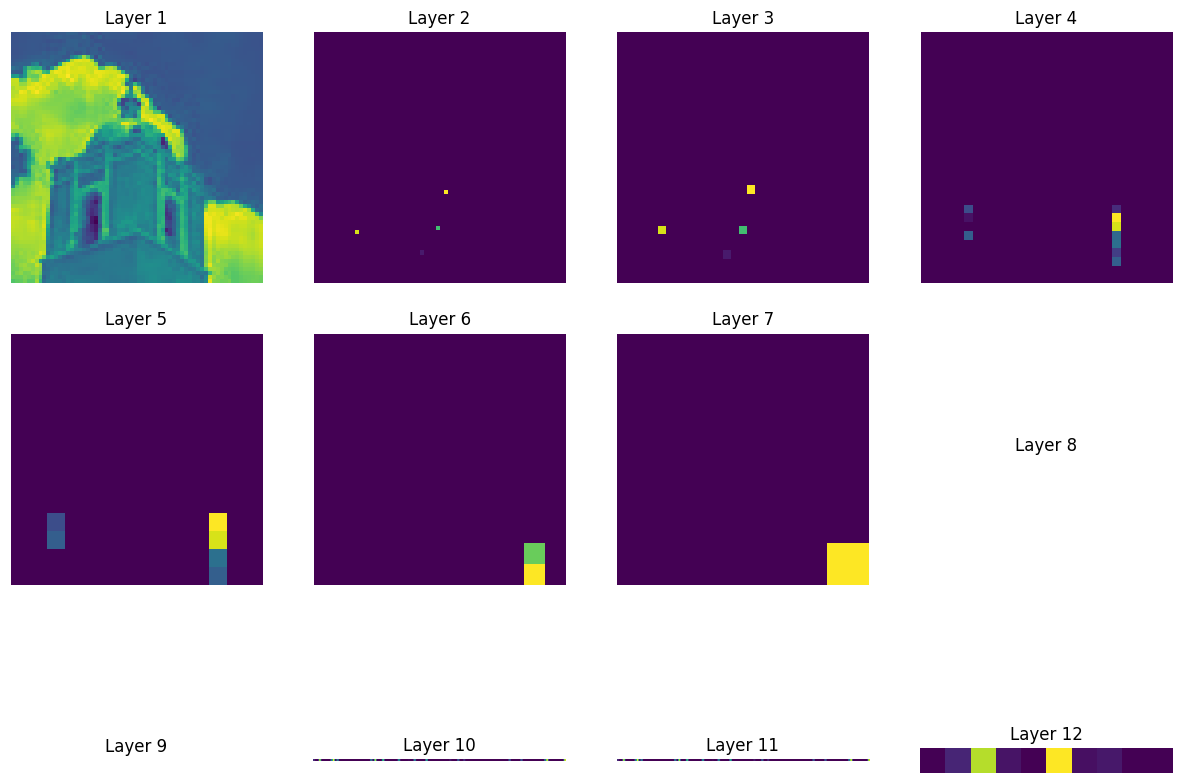
\includegraphics[width=0.8\textwidth]{output.png}
    \caption{Model Layers}
\end{figure}


\subsection{Model Evaluation}
The model's performance was evaluated on a separate test set. The key metrics used for evaluation include accuracy, precision, recall, and F1-score. A confusion matrix was generated to provide detailed insights into the model's classification performance across different categories.

\begin{figure}[H]
    \centering
    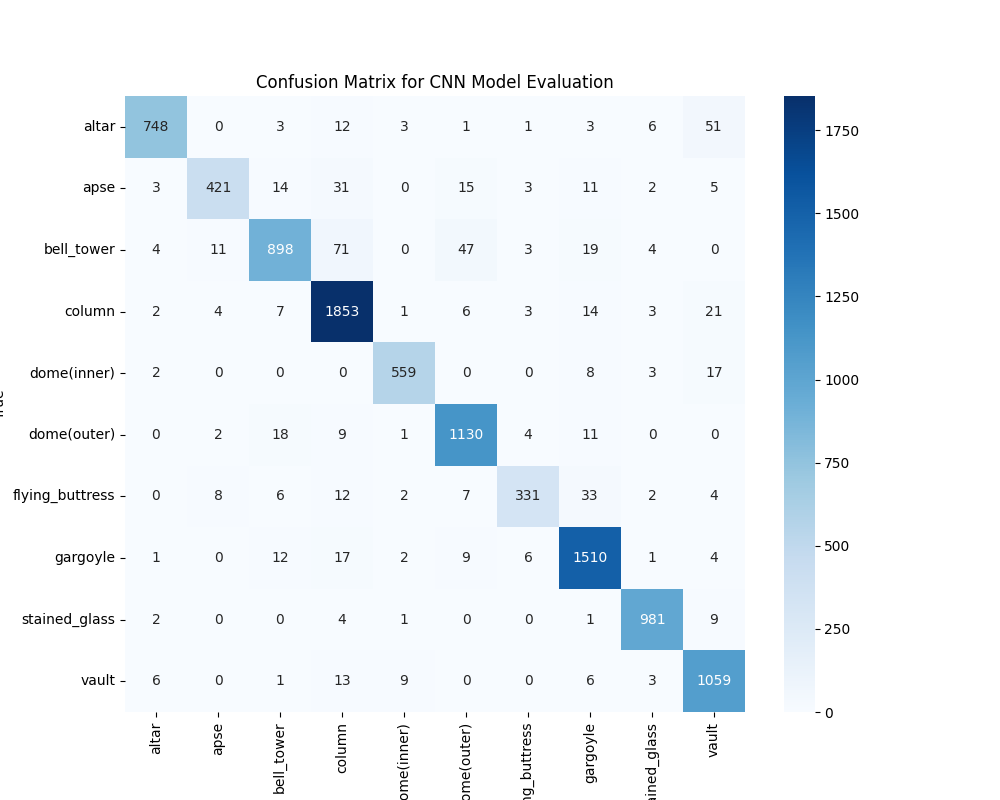
\includegraphics[width=0.8\textwidth]{confusion_matrix.png}
    \caption{Confusion Matrix for CNN Model Evaluation}
\end{figure}

\section{Results}
The model achieved a high accuracy in classifying architectural heritage elements. The confusion matrix above shows the classification performance across all categories. The model performed particularly well on categories like "Vault" and "Column," but there was some misclassification in categories like "Apse" and "Dome (Inner)."

\subsection{Feature Map Visualization}
To gain deeper insights into how the CNN model processes images, we visualized the feature maps generated by the first convolutional layer. These feature maps highlight the areas of the image that the model focuses on while making classification decisions.

\begin{figure}[H]
    \centering
    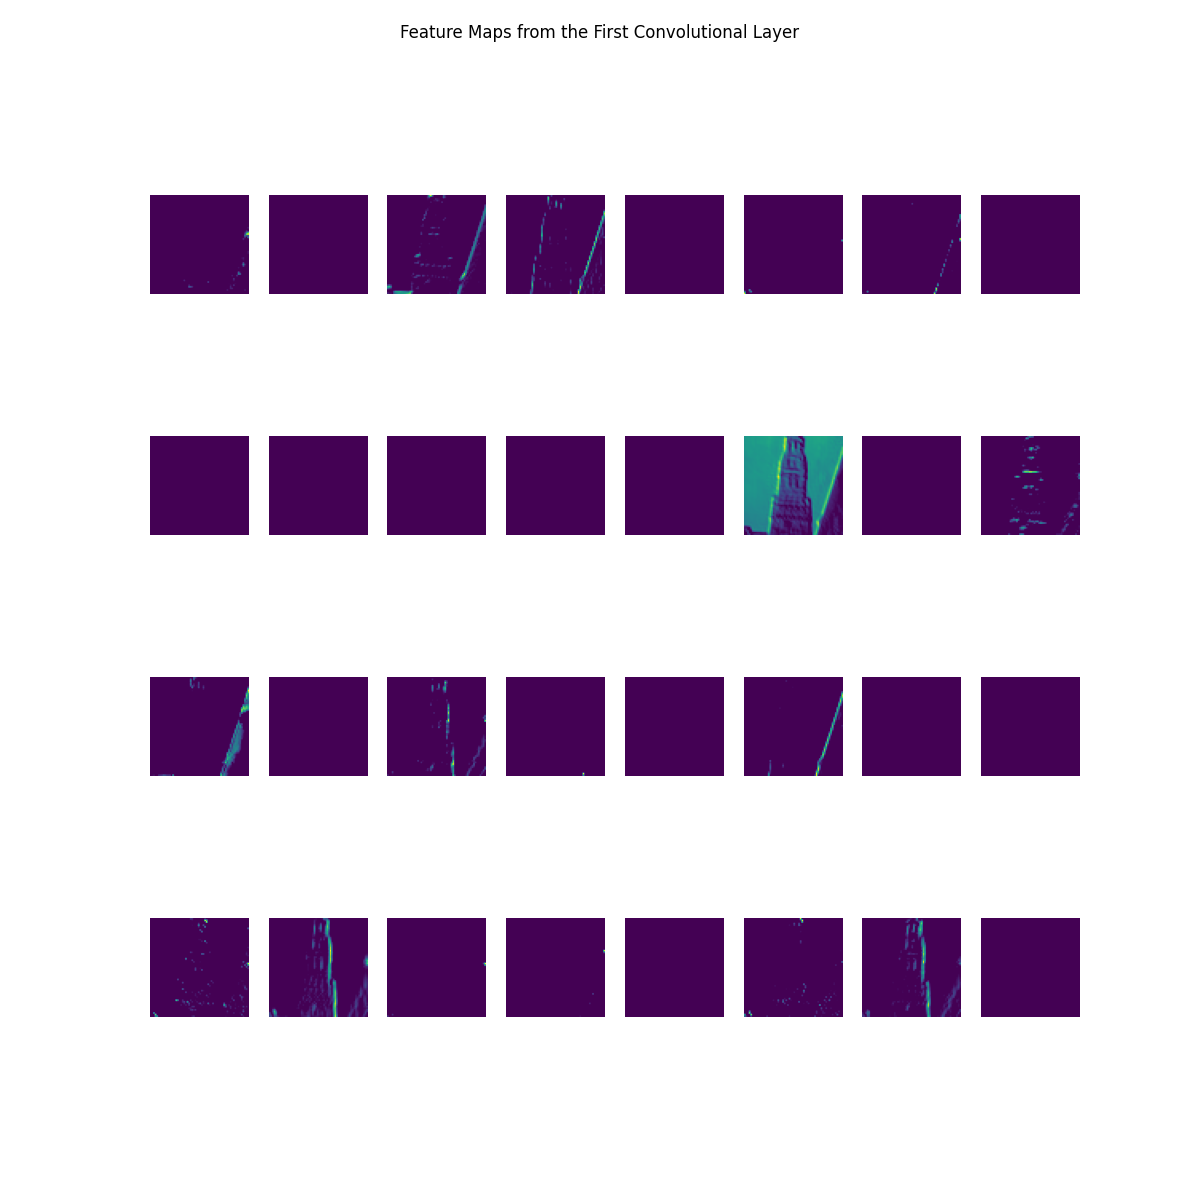
\includegraphics[width=0.8\textwidth]{feature_maps_layer1.png}
    \caption{Feature Maps from the First Convolutional Layer}
\end{figure}

The feature maps reveal that the model is learning to detect low-level features such as edges and textures, which are essential for distinguishing between different architectural elements.

\section{Discussion}
The performance of the CNN model was evaluated through the confusion matrix and the feature map visualizations. The confusion matrix shows that while the model performs well, there is room for improvement in certain categories, especially in the cases of "Apse" and "Dome (Inner)." These misclassifications can be attributed to the similarity between some categories and the limitations of the model's ability to distinguish fine-grained features.

The feature map visualizations provide valuable insight into the areas of the image that the model focuses on. This can help in interpreting the decisions made by the model and may guide further improvements in the model architecture or training process.

\section{Conclusion}
In this project, we successfully trained a CNN model to classify images from the "Architectural Heritage Elements Image64" dataset. The model's performance was evaluated using a confusion matrix, and the feature maps generated by the first convolutional layer were visualized. The results show that the CNN model is effective in classifying architectural elements, although there are opportunities for further refinement. Future work can explore techniques such as transfer learning, deeper architectures, and fine-tuning to improve classification performance.

\section{References}
\begin{itemize}
    \item \href{https://www.kaggle.com/datasets/ikobzev/architectural-heritage-elements-image64-dataset}{Architectural Heritage Elements Image64 Dataset}
    \item \href{https://pytorch.org/docs/stable/index.html}{PyTorch Documentation}
\end{itemize}


\end{document}
